% /**
%  * A template for homework files in math classes. The 
%  * packages and newcommands are a good starting point.
%  *
%  * Author: James K. Pringle
%  * E-mail: jameskpringle@gmail.com
%  * Last Changed: 5 September 2013
%  *
%  * "LaTeX countains the increasing union of MS Word"
%  */
%~~~~~~~~~~~~~~~~~~~~~~~~~~~~~~~~~~~~~~~~~~~~~~~~~~~~~~~~~%
%%%%%%%%%%%%%%%%%%%%%%%%%%%%%%%%%%%%%%%%%%%%%%%%%%%%%%%%%%%
%                                                         %
%                        PAGE SETUP                       %
%                                                         %
%%%%%%%%%%%%%%%%%%%%%%%%%%%%%%%%%%%%%%%%%%%%%%%%%%%%%%%%%%%
\documentclass[letterpaper, 12pt]{article}\usepackage[]{graphicx}\usepackage[]{color}
%% maxwidth is the original width if it is less than linewidth
%% otherwise use linewidth (to make sure the graphics do not exceed the margin)
\makeatletter
\def\maxwidth{ %
  \ifdim\Gin@nat@width>\linewidth
    \linewidth
  \else
    \Gin@nat@width
  \fi
}
\makeatother

\definecolor{fgcolor}{rgb}{0.345, 0.345, 0.345}
\newcommand{\hlnum}[1]{\textcolor[rgb]{0.686,0.059,0.569}{#1}}%
\newcommand{\hlstr}[1]{\textcolor[rgb]{0.192,0.494,0.8}{#1}}%
\newcommand{\hlcom}[1]{\textcolor[rgb]{0.678,0.584,0.686}{\textit{#1}}}%
\newcommand{\hlopt}[1]{\textcolor[rgb]{0,0,0}{#1}}%
\newcommand{\hlstd}[1]{\textcolor[rgb]{0.345,0.345,0.345}{#1}}%
\newcommand{\hlkwa}[1]{\textcolor[rgb]{0.161,0.373,0.58}{\textbf{#1}}}%
\newcommand{\hlkwb}[1]{\textcolor[rgb]{0.69,0.353,0.396}{#1}}%
\newcommand{\hlkwc}[1]{\textcolor[rgb]{0.333,0.667,0.333}{#1}}%
\newcommand{\hlkwd}[1]{\textcolor[rgb]{0.737,0.353,0.396}{\textbf{#1}}}%

\usepackage{framed}
\makeatletter
\newenvironment{kframe}{%
 \def\at@end@of@kframe{}%
 \ifinner\ifhmode%
  \def\at@end@of@kframe{\end{minipage}}%
  \begin{minipage}{\columnwidth}%
 \fi\fi%
 \def\FrameCommand##1{\hskip\@totalleftmargin \hskip-\fboxsep
 \colorbox{shadecolor}{##1}\hskip-\fboxsep
     % There is no \\@totalrightmargin, so:
     \hskip-\linewidth \hskip-\@totalleftmargin \hskip\columnwidth}%
 \MakeFramed {\advance\hsize-\width
   \@totalleftmargin\z@ \linewidth\hsize
   \@setminipage}}%
 {\par\unskip\endMakeFramed%
 \at@end@of@kframe}
\makeatother

\definecolor{shadecolor}{rgb}{.97, .97, .97}
\definecolor{messagecolor}{rgb}{0, 0, 0}
\definecolor{warningcolor}{rgb}{1, 0, 1}
\definecolor{errorcolor}{rgb}{1, 0, 0}
\newenvironment{knitrout}{}{} % an empty environment to be redefined in TeX

\usepackage{alltt}

% 1in margins all the way around
\usepackage[margin=1in]{geometry}

% Sets \parindent to 0 and \parskip to stretchable.
\usepackage{parskip}
% Use for bigger spaces between paragraphs.
%\parskip=1.5\baselineskip

% Set headers and footers
\usepackage{fancyhdr}
\pagestyle{fancy}
% Header
\renewcommand{\headrulewidth}{0.4pt}
\lhead{\textsc{\mathclass}}
\chead{\textsc{\today}}
\rhead{\textsc{\mynamehdr}}
% Footer
\renewcommand{\footrulewidth}{0.4pt}
\lfoot{}
\cfoot{\thepage}
\rfoot{}

% Make the space between lines slightly more generous 
% than normal single spacing, but compensate so that the 
% spacing between rows of matrices still looks normal.  
% Note that 1.1=1/.9090909...
\renewcommand{\baselinestretch}{1.1}
\renewcommand{\arraystretch}{.91}

%%%%%%%%%%%%%%%%%%%%%%%%%%%%%%%%%%%%%%%%%%%%%%%%%%%%%%%%%%%
%                                                         %
%                      USEFUL PACKAGES                    %
%                                                         %
%%%%%%%%%%%%%%%%%%%%%%%%%%%%%%%%%%%%%%%%%%%%%%%%%%%%%%%%%%%

% The classic three
\usepackage{amsmath,amsthm,amssymb}

% Define \newtheorem for use
% No numbers, labeled 'Theorem'
\newtheorem*{nthm}{Theorem}

% Not sure what this is for
\usepackage{amsfonts}

% Fancy script font
\usepackage{mathrsfs}

% Makes enumerate environment much easier to customize
% by specifying the counter
\usepackage{enumerate}

% Color
\usepackage{color}
\usepackage[usenames,dvipsnames,svgnames,table]{xcolor}

% URL links
\usepackage{hyperref}

% For inserting graphics and images
\usepackage{graphicx}
\usepackage{float}
\usepackage[footnotesize]{caption}



%%%%%%%%%%%%%%%%%%%%%%%%%%%%%%%%%%%%%%%%%%%%%%%%%%%%%%%%%%%
%                                                         %
%                   USER-DEFINED COMMANDS                 %
%                                                         %
%%%%%%%%%%%%%%%%%%%%%%%%%%%%%%%%%%%%%%%%%%%%%%%%%%%%%%%%%%%

% Make a hyperlink with colored text
\newcommand{\hrefcolor}[3]{\href{#1}{\textcolor{#3}{#2}}}

% Make a hyperlink with gray text
\newcommand{\hrefgray}[2]{\hrefcolor{#1}{#2}{Gray}}

% Make the header for the first page
\newcommand{\firstpageinfo}{
\textsf{
\begin{flushleft}
\sc \myname \\
\normalfont \mathclass \\
\professorname \\
\assignmentnumber \\
\thedate
\end{flushleft}
} \bigskip
}

% Make problem list for "title" of page
\newcommand{\problemlist}{ 
\begin{center}
\textbf{\Large \textsf{\assignmentnumber}}\\
\textit{\textsf{\problemset}}
\end{center}
\bigskip
}

%~~~~~~~~~~~~~~~~~~~~~~~~~~~~~~~~~~~~~~~~~~~~~~~~~~~~~~~~~%
%                                                         %
%               LETTERS, FUNCTIONS, AND TEXT              %
%                                                         %
%~~~~~~~~~~~~~~~~~~~~~~~~~~~~~~~~~~~~~~~~~~~~~~~~~~~~~~~~~%

% A
\newcommand{\cA}{\mathcal{A}}
\newcommand{\sA}{\mathscr{A}}
\renewcommand{\aa}{\;\text{a.a.}}
\renewcommand{\ae}{\;\text{a.e.}}
% B
\newcommand{\B}{\mathscr{B}}
\newcommand{\cB}{\mathcal{B}}
% C
\newcommand{\cC}{\mathcal{C}}
\newcommand{\cov}{\text{cov}}
% E
\newcommand{\E}{\mathbb{E}}
% F
\newcommand{\sF}{\mathscr{F}}
\newcommand{\cF}{\mathcal{F}}
\newcommand{\Ft}{F^\sim}
% G
\newcommand{\cG}{\mathcal{G}}
\newcommand{\sG}{\mathscr{G}}
% H
\newcommand{\bh}{\mathbf{h}}
% I
\newcommand{\io}{\;\text{i.o.}}
% N
\newcommand{\N}{\mathbb{N}}
% P
\newcommand{\cP}{\mathcal{P}}
\newcommand{\sP}{\mathscr{P}}
\newcommand{\pr}{\text{pr}}
% Q
\newcommand{\Q}{\mathbb{Q}}
% R
\newcommand{\R}{\mathbb{R}}
\newcommand{\bR}{\mathbf{R}}
\newcommand{\cR}{\mathcal{R}}
% S
\newcommand{\cS}{\mathcal{S}}
% U
\newcommand{\cU}{\mathcal{U}}
% V
\newcommand{\var}{\text{var}}
% Z
\newcommand{\Z}{\mathbb{Z}}
% Punctuation
\newcommand{\sbs}{\;|\;} % space bar space
% Math
\newcommand{\imii}{\int_{-\infty}^\infty}
\newcommand{\pion}{\prod_{i=1}^n}
\newcommand{\pioI}{\prod_{i=1}^I}
\newcommand{\pjon}{\prod_{j=1}^n}
\newcommand{\pjoJ}{\prod_{j=1}^J}
\newcommand{\pkon}{\prod_{k=1}^n}
\newcommand{\pkoK}{\prod_{k=1}^K}
\newcommand{\sion}{\sum_{i=1}^n}
\newcommand{\sioI}{\sum_{i=1}^I}
\newcommand{\sjon}{\sum_{j=1}^n}
\newcommand{\sjoJ}{\sum_{j=1}^J}
\newcommand{\skon}{\sum_{k=1}^n}
\newcommand{\skoK}{\sum_{k=1}^K}
\newcommand{\sioi}{\sum_{i=1}^\infty}
\newcommand{\sjoi}{\sum_{j=1}^\infty}
\newcommand{\skoi}{\sum_{k=1}^\infty}
\newcommand{\sio}{\sum_{i=1}}
\newcommand{\sjo}{\sum_{j=1}}
\newcommand{\sko}{\sum_{k=1}}
% Typography
\newcommand{\scb}[1]{\textsc{\textbf{#1}}}

%~~~~~~~~~~~~~~~~~~~~~~~~~~~~~~~~~~~~~~~~~~~~~~~~~~~~~~~~~%
%                                                         %
%            CHANGE THESE BASED ON THE PAPER              %
%                                                         %
%~~~~~~~~~~~~~~~~~~~~~~~~~~~~~~~~~~~~~~~~~~~~~~~~~~~~~~~~~%

% Constants for fancy header and first page info
\newcommand{\mynamehdr}{\hrefgray{http://biostat.jhsph.edu/~jpringle/}{\myname}}
\newcommand{\mathclass}{140.663 Geostatistics}
\newcommand{\myname}{James K. Pringle}
\newcommand{\professorname}{Dr. Curriero}
\newcommand{\assignmentnumber}{Assignment 2}
\newcommand{\thedate}{\today}
\newcommand{\problemset}{Questions 2-4}

%%%%%%%%%%%%%%%%%%%%%%%%%%%%%%%%%%%%%%%%%%%%%%%%%%%%%%%%%%%
%                                                         %
%                      BEGIN DOCUMENT                     %
%                                                         %
%%%%%%%%%%%%%%%%%%%%%%%%%%%%%%%%%%%%%%%%%%%%%%%%%%%%%%%%%%%
\IfFileExists{upquote.sty}{\usepackage{upquote}}{}
\begin{document}

% Take header off of first page
\thispagestyle{empty}

% Put in first page info (top of page)
\firstpageinfo

% Put in title for the paper
\problemlist

%%%%%%%%%%%%%%%%%%%%%%%%%%%%%%%%%%%%%%%%%%%%%%%%%%%%%%%%%%%
%                                                         %
%                     Start Problem 1                     %
%                                                         %
%%%%%%%%%%%%%%%%%%%%%%%%%%%%%%%%%%%%%%%%%%%%%%%%%%%%%%%%%%%
\setcounter{section}{1}
\section{Large Scale vs. Small Scale Spatial Variation}
The data file \texttt{Q2 Data.csv} has 6 variables with 200 records. Variables $y_1$ and $y_2$ are two simulated spatial data sets (outcome variables) with coordinates $coordx$ and $coordy$. The variables $x_1$ and $x_2$ are potential explanatory variables or covariates for each outcome respectively.

\begin{enumerate}[(a)]
\item
Read the data file \texttt{Q2 Data.csv} into your current \texttt{R} session using the \texttt{read.csv} command.

\textsf{Done}.
\item
Perform some exploratory spatial data analysis on the variables $y_1$ and $y_2$ with focus on large scale spatial variation and interpret your findings. Recall in the spatial literature, the terms large scale and small scale spatial variation are often taken to mean first order and second order variation.



\begin{knitrout}
\definecolor{shadecolor}{rgb}{0.969, 0.969, 0.969}\color{fgcolor}
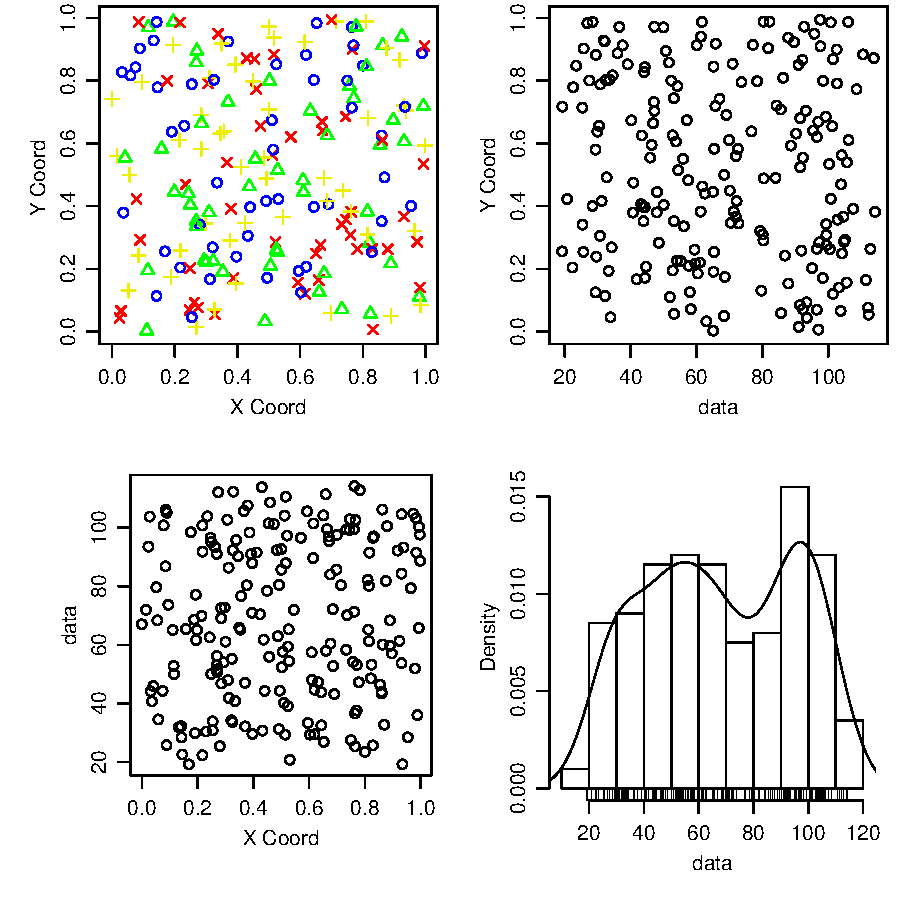
\includegraphics[width=\maxwidth]{figure/plot1} 

\end{knitrout}

\begin{knitrout}
\definecolor{shadecolor}{rgb}{0.969, 0.969, 0.969}\color{fgcolor}
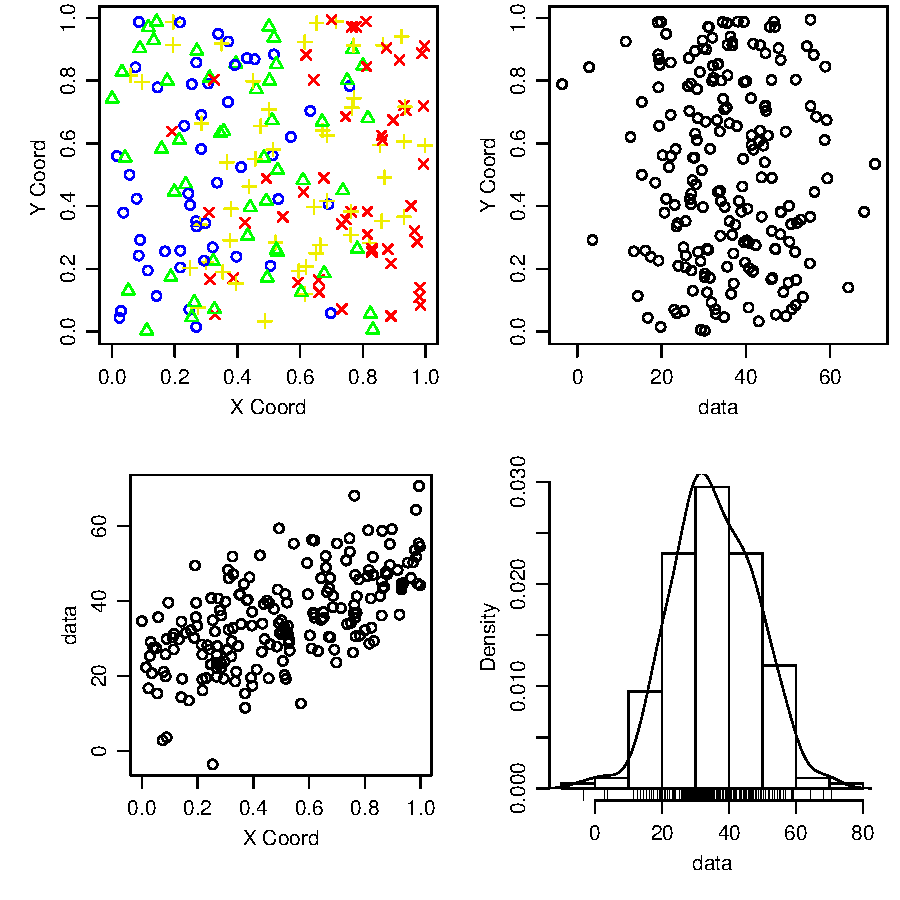
\includegraphics[width=\maxwidth]{figure/plot2} 

\end{knitrout}



{\sf
We do not have covariates other than the $x$ and $y$ coordinates. Therefore the plot of Data vs. $x$-coordinate and $y$-coordinate vs Data should be sufficient to describe the large scale variation. In the first set of plots, it does not appear that there is any trend between either $x$- or $y$-coordinate with the data. The scatterplots appear to be a blob of uncorrelated points. This would indicate that there is not any large scale spatial variation.

There is a difference in the second set of plots in that the $x$-coordinate seems to have a linear relationship with the data. That means that there is large scale variation with the covariates available.}

\item
Continue from (b) above and explore small scale spatial variation. Estimate and plot semivariograms for $y_1$ and $y_2$. Interpret results from both (b) and (c).

\begin{knitrout}
\definecolor{shadecolor}{rgb}{0.969, 0.969, 0.969}\color{fgcolor}
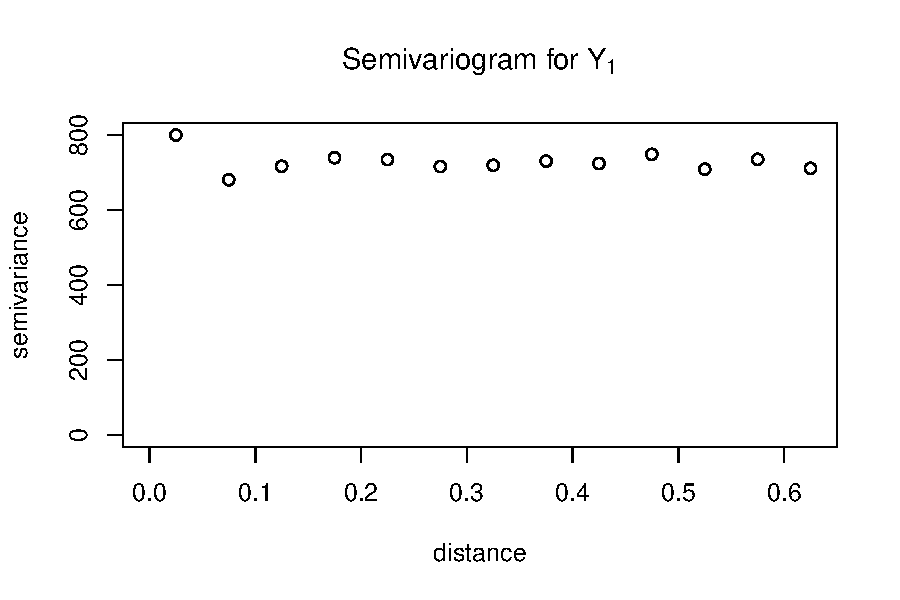
\includegraphics[width=\maxwidth]{figure/unnamed-chunk-1} 

\end{knitrout}

\begin{knitrout}
\definecolor{shadecolor}{rgb}{0.969, 0.969, 0.969}\color{fgcolor}
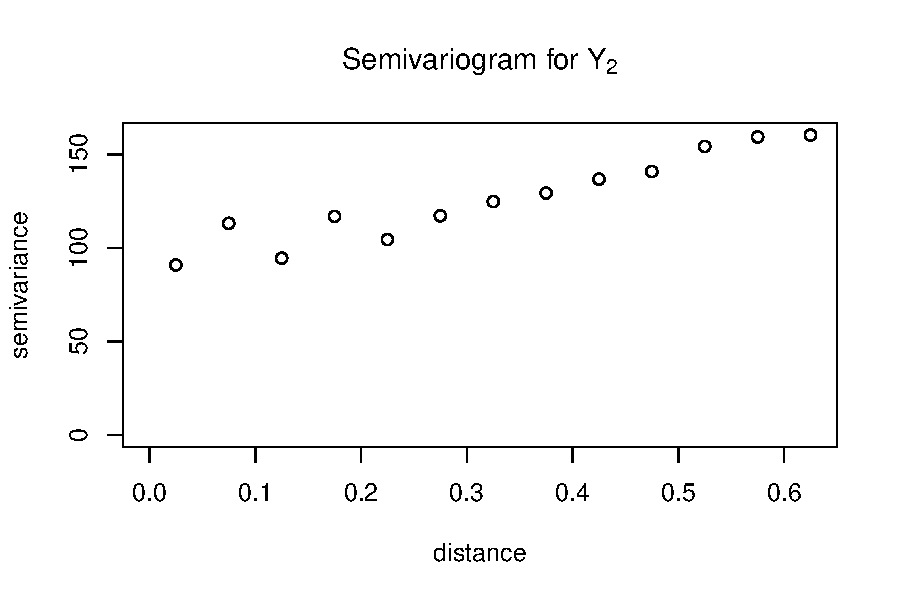
\includegraphics[width=\maxwidth]{figure/unnamed-chunk-2} 

\end{knitrout}


{\sf
The variogram for $y_1$ is a flat line. This implies that $y_1$ is not spatially dependent, or that any spatial dependence is dwarfed by (is much smaller in comparison to) the variance of the data. From the plots in (b), the $y_1$ values seem pretty uniformly scattered throughout the domain.
 
The variagram for $y_2$ shows an increasing trend. This implies spatial dependence, that points closer together have more similar values than points farther apart. This reinforces the notion that there is large scale variation associated with the $x$-coordinate as discussed in (b).}

\item
Perform simple linear regressions for $y_1$ using $x_1$ as a covariate and for $y_2$ using $x_2$ as the covariate. Estimate and plot the residual semivariograms for each. Interpret.

\begin{knitrout}
\definecolor{shadecolor}{rgb}{0.969, 0.969, 0.969}\color{fgcolor}
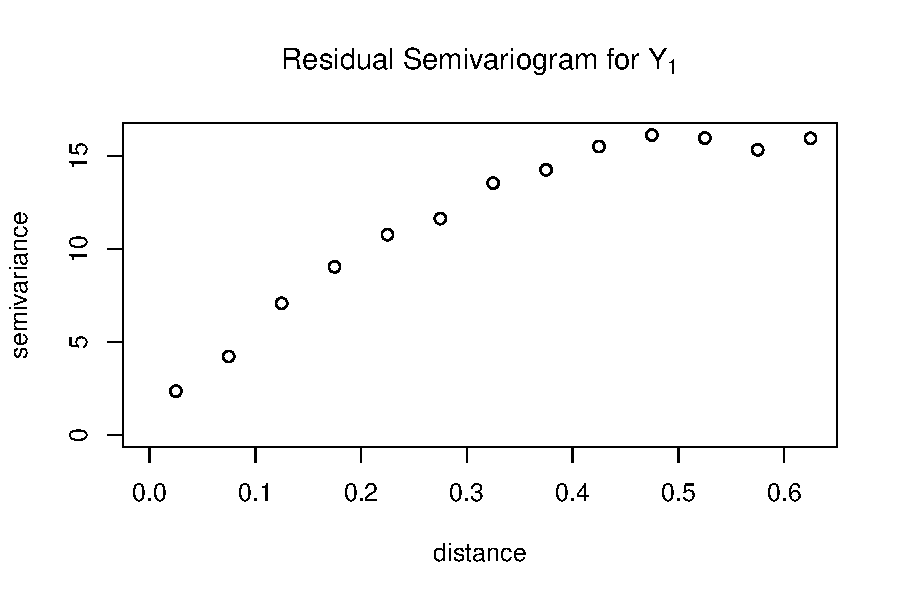
\includegraphics[width=\maxwidth]{figure/unnamed-chunk-3} 

\end{knitrout}

\begin{knitrout}
\definecolor{shadecolor}{rgb}{0.969, 0.969, 0.969}\color{fgcolor}
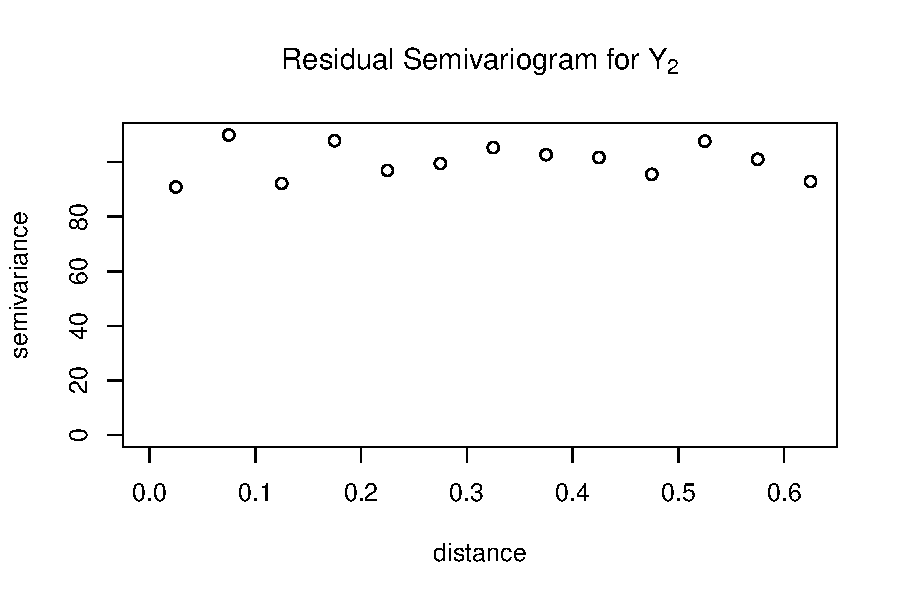
\includegraphics[width=\maxwidth]{figure/unnamed-chunk-4} 

\end{knitrout}


{\sf
For $Y_1$, the residuals show spatial dependence. In imprecise terms, after accounting for the variation of $X_1$, the left over variation (small scale variation) is spatially dependent. Since the variagram of $Y_1$ is a flat line, it may be possible to conclude that variation due to $X_1$ is much larger than the spatial variance.

The variogram of the residuals of $Y_2$ is flat. For $Y_2$, after accounting for the variation due to $X_2$ (the $x$-coordinate), there is no evidence of spatial dependence in the residuals. This means there is no small scale spatial variation in the data, that the data has only large scale spatial variation.
}


\item
Below are the statistical models used to simulate these data,
\begin{align*}
Y_1(s) 
&= 20+3X_1(s)+\epsilon_1(s), 
&\epsilon_1(s)\sim N(0,\sigma_1^2) 
\quad
& corr(\epsilon_1(s_i),\epsilon_1(s_j)) \neq 0
\\
Y_2(s) 
&= 20+3X_2(s)+\epsilon_2(s), 
&\epsilon_2(s)\sim N(0,\sigma_2^2) 
\quad
& corr(\epsilon_2(s_i),\epsilon_2(s_j)) = 0,
\end{align*}
where coordinates $s = (coordx, coordy)$, $X_1(s)$ are uniform random numbers generated independent of $Y_1$, $X_2(s)$ are actually the \textit{coordx} values scaled up by a factor of 10, $\epsilon_1(s)$ is a spatially dependent Normal random variable, and $\epsilon_2(s)$ is a Normal random variable spatially independent. Thus $Y_1(s)$ is generated from adding a spatially unstructured variable $X_1(s)$ to spatially structured errors $\epsilon_1(s)$. In contrast, $Y_2(s)$ is generated from adding a spatially structured variable $X_2(s)$ to spatially unstructured errors $\epsilon_2(s)$. With this knowledge, comment on the behavior of the respective semivariograms of the outcome variables compared to their respective residual semivariograms. That is compare the spatial dependence structure of $Y_1$ with the spatial dependence of the residuals from the regression of $Y_1$ on $X_1$, and the spatial dependence of $Y_2$ with the spatial dependence of the residuals from the regression of $Y_2$ on $X_2$.

{\sf
Given this knowledge of how the outcome variables $Y_1$ and $Y_2$ are simulated, it is easier to interpret the variograms. The variogram of $Y_1$ appears to indicate no spatial variation. That is because the magnitude of the large scale component is much larger than the magnitude of the spatially structured errors. Therefore, after regression onto $X_1$, the residuals reveal the spatially structured nature of the errors. That is why the variogram of the residuals $Y_1$ are spatially dependent.

The variogram of $Y_2$ shows spatial dependence because it is built into the $Y_2$ by means of $X_2$ (the $x$-coordinate). After regression onto $X_2$, the residuals reveal the spatially independent nature of the errors. This is seen by the flat trend in the variogram of the residuals.
}
\end{enumerate}

\section{Understanding the Covariance Matrix}
Consider the following spatial design of locations.

\begin{verbatim}
Location   (x,y)
----------------
         1 (1,1)
         2 (1,2)
         3 (1,3)
         4 (2,1)
         5 (2,2)
         6 (2,3)
         7 (3,1)
         8 (3,2)
         9 (3,3)
----------------
\end{verbatim}

Let’s assume we know the spatial dependance for this design is characterized by an exponential semivariogram with nugget of zero, sill of 25, and range of 2,
\[
\gamma(h) = 25 (1 - \exp(-h/2)).
\]
\begin{enumerate}[a.]
\item
Use the known semivariogram model and the relation $γ(\|h\|) = C(0) - C(\|h\|)$ to estimate the covariogram $C(\|h\|)$ and correlogram $\rho(\|h\|)$. Also provide estimates for the variogram and the number of data points falling within each distance class $N(\|h\|)$. The table on the following page is provided to fill in and to further clarify what is being asked. The sample locations from this $3 \times 3$ regular grid were used to dictate the distance classes.




\begin{tabular}{c c c c c c}
Distance & & Variogram & Semivariogram & Covariogram & Correlogram
\\
$\|\bh \|$ & $N(\|\bh \|)$ & $2 \gamma(\|\bh \|)$ & $\gamma(\|\bh \|)$ & $C(\|\bh \|)$ & $\rho(\|\bh \|)$
\\
\hline \hline 
 1 & 12 & 19.673 & 9.837 & 15.163 & 0.607 \\
 1.414 & 8 & 25.344 & 12.672 & 12.328 & 0.493 \\
 2 & 6 & 31.606 & 15.803 & 9.197 & 0.368 \\
 2.236 & 8 & 33.653 & 16.827 & 8.173 & 0.327 \\
 2.828 & 2 & 37.842 & 18.921 & 6.079 & 0.243

\\
\hline
\hline
\end{tabular}


\item
Use results from the completed table as well as the spatial design of these 9 locations to fill in values for the distance matrix and the covariance matrix $\Sigma$. Empty $9 \times 9$ matrices (with 81 entries) are provided for convenience. View these matrices as each having 9 rows and 9 columns for spatial locations 1 to 9 and cross reference accordingly. For example, row 3 column 5 corresponds to the location 3 location 5 pair.





\[
\text{Distance} = \begin{bmatrix}
 0 & 1 & 2 & 1 & 1.414 & 2.236 & 2 & 2.236 & 2.828 \\
 1 & 0 & 1 & 1.414 & 1 & 1.414 & 2.236 & 2 & 2.236 \\
 2 & 1 & 0 & 2.236 & 1.414 & 1 & 2.828 & 2.236 & 2 \\
 1 & 1.414 & 2.236 & 0 & 1 & 2 & 1 & 1.414 & 2.236 \\
 1.414 & 1 & 1.414 & 1 & 0 & 1 & 1.414 & 1 & 1.414 \\
 2.236 & 1.414 & 1 & 2 & 1 & 0 & 2.236 & 1.414 & 1 \\
 2 & 2.236 & 2.828 & 1 & 1.414 & 2.236 & 0 & 1 & 2 \\
 2.236 & 2 & 2.236 & 1.414 & 1 & 1.414 & 1 & 0 & 1 \\
 2.828 & 2.236 & 2 & 2.236 & 1.414 & 1 & 2 & 1 & 0\end{bmatrix}\]



\[
\Sigma = \begin{bmatrix}
 25 & 15.163 & 9.197 & 15.163 & 12.328 & 8.173 & 9.197 & 8.173 & 6.079 \\
 15.163 & 25 & 15.163 & 12.328 & 15.163 & 12.328 & 8.173 & 9.197 & 8.173 \\
 9.197 & 15.163 & 25 & 8.173 & 12.328 & 15.163 & 6.079 & 8.173 & 9.197 \\
 15.163 & 12.328 & 8.173 & 25 & 15.163 & 9.197 & 15.163 & 12.328 & 8.173 \\
 12.328 & 15.163 & 12.328 & 15.163 & 25 & 15.163 & 12.328 & 15.163 & 12.328 \\
 8.173 & 12.328 & 15.163 & 9.197 & 15.163 & 25 & 8.173 & 12.328 & 15.163 \\
 9.197 & 8.173 & 6.079 & 15.163 & 12.328 & 8.173 & 25 & 15.163 & 9.197 \\
 8.173 & 9.197 & 8.173 & 12.328 & 15.163 & 12.328 & 15.163 & 25 & 15.163 \\
 6.079 & 8.173 & 9.197 & 8.173 & 12.328 & 15.163 & 9.197 & 15.163 & 25\end{bmatrix}\]




\item
Answer the following
\begin{enumerate}[(i)]
\item
In this example what would be the covariance between data that are separated by a distance of 2.236?

\textsf{The covariance of data separated by $2.236$ is $8.173$, as can be seen by the table in ``a.''}
\item
What would be the covariance between data at location 1 and location 7?

\textsf{The covariance between the data at location 1 and location 7 is equal to $\Sigma_{17}$ and $\Sigma_{71}$, which is $9.197$.}
\item
What is the variance represented by this semivariogram?

\textsf{The variance represented by this semivariogram is the variance of the data, $\var(Z(s))$. According to class lecture (slides 85, 104), $\var(Z(s)) = C(0) = \tau^2 + \sigma^2$. So the variance of the data is the total sill, i.e. 25.}
\item
Based on the known semivariogram, at what distance would points become approximately uncorrelated?

\textsf{For exponential semivariograms, the $3\phi$ is the distance where points become approximately uncorrelated, where $\phi$ is the range (see slide 100). Here $3\phi = 3\cdot 2= 6
$}
\end{enumerate}
\item
Now suppose we assumed for this design that the data were independent with variance 25. Fill in the entries of the covariance matrix $\Sigma$. A second empty $9 \times 9$ matrix is provided for convenience.

{\sf
If the data are assumed independent, then cov$(Z(s_i),Z(s_j)) = 0$ where $s_i \neq s_j$. Hence,
}


\[
\Sigma = \begin{bmatrix}
 25 & 0 & 0 & 0 & 0 & 0 & 0 & 0 & 0 \\
 0 & 25 & 0 & 0 & 0 & 0 & 0 & 0 & 0 \\
 0 & 0 & 25 & 0 & 0 & 0 & 0 & 0 & 0 \\
 0 & 0 & 0 & 25 & 0 & 0 & 0 & 0 & 0 \\
 0 & 0 & 0 & 0 & 25 & 0 & 0 & 0 & 0 \\
 0 & 0 & 0 & 0 & 0 & 25 & 0 & 0 & 0 \\
 0 & 0 & 0 & 0 & 0 & 0 & 25 & 0 & 0 \\
 0 & 0 & 0 & 0 & 0 & 0 & 0 & 25 & 0 \\
 0 & 0 & 0 & 0 & 0 & 0 & 0 & 0 & 25\end{bmatrix}\]

\end{enumerate}


\section{The Wolfcamp Aquifer Data}

This data is already in R. Typing the commands \texttt{data(wolfcamp)} and \texttt{help(wolfcamp)} will load the data and show a brief description. The article \textit{Geostatistics} by N. Cressie 1989 \textit{American Statistician}, 43, 197-202 posted on the course website will provide some background. R commands that produce all output required is provided separately. Use these as a guide in generating other results or graphs you wish.

\begin{enumerate}[a.]
\item
Review the article \textit{Geostatistics} by Cressie. This is not necessarily an easy read but focus on the Introduction, Section on the case study, Concluding Remarks, and the general methodology he proposed to krige this data. See the answer to (b) below to help with understanding the read.

\item
Describe the modeling approach used by Cressie to krige the Wolfcamp Aquifer data. Be specific to discuss large scale and small scale variation and any assumptions made about each. I would suggest writing out a model with descriptions (like those shown in class) that depicts Cressie’s approach. Answer below.

{\sf
It appears that Cressie is only estimating the data $Y(s)$ (piezometric-head data) through the variogram (no covariates). This is equivalent to 
\[
Y(s) = b_0 + \epsilon(s)
\]
However, the error terms have a more complicated structure than what we have discussed in class. Here, the process is modeled to show anisotropy. The variogram of the data is a mixture of ``variograms'' in two different directions (with tolerance in the direction).
}

\item
Perform some exploratory spatial data analysis, both with a focus on large scale and small scale variation.

\begin{knitrout}
\definecolor{shadecolor}{rgb}{0.969, 0.969, 0.969}\color{fgcolor}
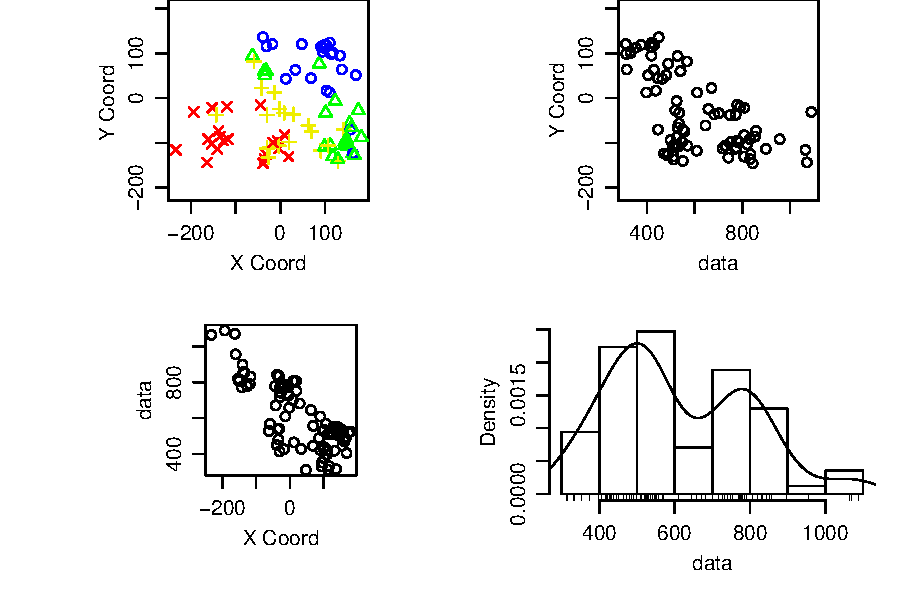
\includegraphics[width=\maxwidth]{figure/wolfcamp2} 

\end{knitrout}

{\sf
According to this plot, there appears to be a trend surface based on the $x$- and the $y$-coordinate. Performing a linear regression on these two covariates (with no interaction) gives

\begin{knitrout}
\definecolor{shadecolor}{rgb}{0.969, 0.969, 0.969}\color{fgcolor}\begin{kframe}
\begin{verbatim}
## 
## Call:
## lm(formula = pressure ~ xcoord + ycoord, data = wolf)
## 
## Residuals:
##     Min      1Q  Median      3Q     Max 
## -111.99  -50.30   -9.33   48.51  197.99 
## 
## Coefficients:
##             Estimate Std. Error t value Pr(>|t|)    
## (Intercept) 607.7707     7.5222    80.8   <2e-16 ***
## xcoord       -1.2784     0.0655   -19.5   <2e-16 ***
## ycoord       -1.1387     0.0774   -14.7   <2e-16 ***
## ---
## Signif. codes:  0 '***' 0.001 '**' 0.01 '*' 0.05 '.' 0.1 ' ' 1
## 
## Residual standard error: 62.3 on 82 degrees of freedom
## Multiple R-squared:  0.891,	Adjusted R-squared:  0.888 
## F-statistic:  335 on 2 and 82 DF,  p-value: <2e-16
\end{verbatim}
\end{kframe}
\end{knitrout}

The effect of both coordinates is a highly significant, negative linear relationship. According to the $R^2$ value, these two covariates explain 62\% of the variation of the data. This shows large scale variation.

However, a variogram of the residuals shows there is still small scale variation.

\begin{knitrout}
\definecolor{shadecolor}{rgb}{0.969, 0.969, 0.969}\color{fgcolor}
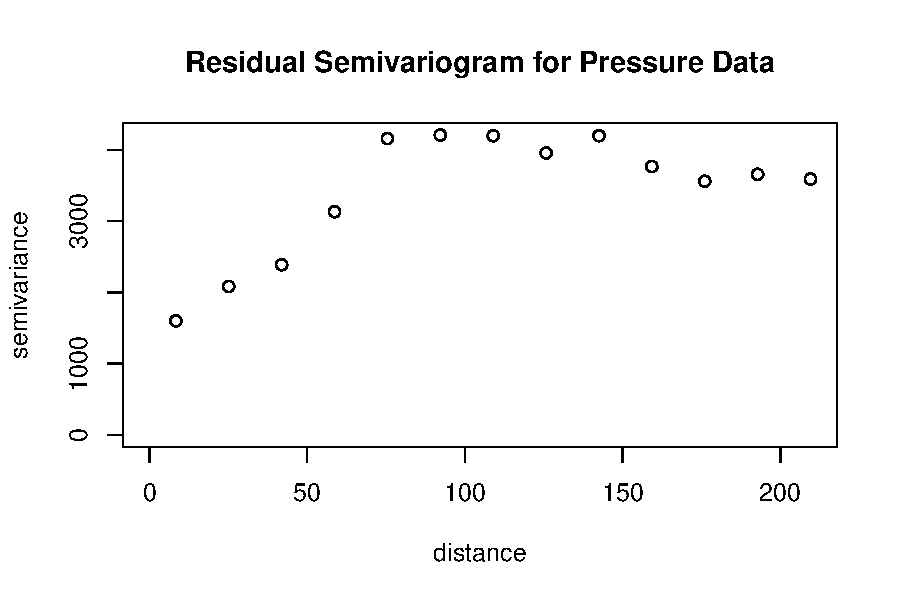
\includegraphics[width=\maxwidth]{figure/resid3} 

\end{knitrout}

}
\item
Suggest an alternative kriging approach than that taken in the article. Again be specific to write out a model with assumptions, etc. that describes your approach. Discuss why you selected this alternative.

{\sf
In my approach, I would try to add covariates for a ``universal kriging'' model. I do not know much about groundwater pressure, but I would think that the elevation of the ground water would be important (and that it would vary spatially). So my model would be
\[
Y(s) = b_0 + b_1 X(s) + \epsilon(s)
\]
where $X(s)$ is the elevation of the groundwater at location $s$. I would still check the ``directional variogram'' like Cressie did, and model it as he did if two directions have different variograms.
}

\item
Is the data available to generate a kriged map of pressure based on your kriging model suggested in (d)? Explain.

{\sf
It appears that the elevation data needed is not stored in R. I do not know what methods exist for finding this elevation, but according to \url{https://water.usgs.gov/edu/gwhowtofind.html}, ``a target area must be thoroughly tested and studied to identify hydrologic and geologic features important to the planning and management of the resource.'' This means that it would be difficult (in time and money) to collect the data I would like to have. 
}

\end{enumerate}

\end{document}
